
\chapter{Desenvolvimento dos protótipos}
% Label para referenciar
\label{desenvolvimento-prototipos}

% Diminuir espaçamento entre título e texto
\vspace{-1.9cm}

% Texto do capítulo

  Este capítulo apresenta o cenário proposto para o estudo de caso, bem
  como o desenvolvimento dos protótipos com suas fases de implementação, iniciando
  pela elicitação dos requisitos seguindo a abordagem \ac{REST}.
  
  Como serão desenvolvidos dois protótipos com o objetivo de compara-los um com o outro,
  iniciaremos o desenvolvimento com o \textit{framework} Django, e por fim, faremos o desenvolvimento
  com o ambiente Node.Js e \textit{framework} Express.Js formando assim a aplicação proposta.
  
\section{O escopo do projeto}
\label{escopo-projeto}

  Com base nos aspectos abordados ao longo deste trabalho, 
  esta seção visa apresentar o desenvolvimento de um Web Service seguindo os padrões \ac{REST} e a utilização 
  de um banco de dados relacional Postgres para a persistência dos dados.
  
  Tal serviço possuirá métodos que serão consumidos por dispositivos clientes.

\subsection{Levantamento Requisitos}
\label{levantamento-requisitos}

  Utilizaremos o mesmo exemplo citado por \citeonline{Pereira:2013} pois é de fácil compreensão
  e entendimento de uma simples aplicação. Em seu livro o autor para ensinar o \textit{framework}
  Express.Js e Node.Js cria uma agenda de contatos integrando-o com um Web \textit{chat} funcionando em tempo-real.
  
  A aplicação do autor possui requisitos funcionais bastante objetivos tais como: O usuário cria, edita ou exclui um contato; 
  o usuário realiza \texit{login} informando nome e e-mail; conectar ou desconectar no chat; poder enviar e receber mensagens no chat somente
  dos contatos \textit{online}
  
  Ao investigar o primeiro requisito -(criar, editar ou excluir um contato)- foi possível encaixa-lo neste trabalho pois um serviço em
  REST encaixa perfeitamente nesta necessidade. Como este trabalho não possui o mesmo foco do aplicativo utilizado por \citeonline{Pereira:2013}
  e sim comparar desempenho das aplicações simplificamos o desenvolvimento para cumprir o objetivo deste trabalho.

\subsubsection{Elicitação de requisitos}

  Sendo assim, é possível destacar os seguintes requisitos candidatos

  \begin{compactitem}
    \item[d)] A \ac{API} \ac{REST} deverá ter um recurso chamado Pessoas.
    \item[e)] A \ac{API} \ac{REST} deverá prover estratégias para manipular as ações de CRUD de uma pessoa(s)
    \item[f)] A \ac{API} \ac{REST} deverá ter um recurso chamado Contatos.
    \item[g)] A \ac{API} \ac{REST} deverá prover estratégias para manipular as ações de CRUD de um contato(s)
  \end{compactitem}
  
\subsubsection{Análise dos requisitos}
  
  Perante os requisitos elicitados verificou-se que o objetivo essencial de uma pessoa, candidato a usuário
  do sistema, é controlar os próprios contatos.
  
  O principal requisito destacado na análise é registrar estes contatos. Para atender o requisito
  propõem-se a utilização de uma \ac{API} \ac{REST}, para fornecer os \ac{CRUD} de cada recurso
  como na Tabela \ref{tab:api-descricao-contato}.
 
  
  \begin{table}[H]
    \centering
    \footnotesize
    \vspace{0.5cm}
    % Alterar espaçamentos antes e depois do caption
    \setlength{\abovecaptionskip}{0pt}
    \setlength{\belowcaptionskip}{0pt}
    % Caption
    \caption[Descrição da API de contatos]{Descrição da API de contatos}
    \label{tab:api-descricao-contato}
    % Conteúdo da tabela
    \begin{tabular}{c|c|c|p{8cm}}
      \hline \hline
      Metódo  &	Parâmetro &	Recurso &	Descrição \\
      \hline \hline
      GET	& -	& contatos	& Retorna a lista de contatos 
					  cadastrados no banco de dados \\
      \hline \hline
    \end{tabular}
    % Fonte
    \captionfont{\small{\textbf{\\Fonte: Autor}}}
  \end{table}
  
\subsubsection{Tecnologias Utilizadas}


  Aplicativo comparativo Django
    
    \begin{compactitem}
      \item[a)] Python – Linguagem de programação OO usada na comparação de aplicativos deste trabalho;
      \item[b)] Postgres – Banco de dados relacional
      \item[c)] Django/django-rest-framework – Framework Django para aplicações web e o pacote django-rest-framework
      para facilitar o desenvolvimento.
    \end{compactitem}
    
  Aplicativo Node.JS
  
    \begin{compactitem}
      \item[a)] Node.Js – Ambiente de Programação Backend para apresentação deste trabalho
      \item[b)] Postgress – Banco de dados relacional
      \item[c)] Express – Framework para aplicações web
    \end{compactitem}
 
\subsubsection{Mapeamento de dados}

  De acordo com os requisitos elicitados foi contruido o diagrama de entidade e relecaionamento para melhor
  documentar estes requisitos.
  
  \begin{figure}[H]
    % Alterar espaçamentos antes e depois do caption
    \setlength{\abovecaptionskip}{0pt}
    \setlength{\belowcaptionskip}{0pt}
    % Caption
    \caption[Diagrama de entidade e relacionamentos]{Diagrama de entidade e relacionamentos}
    \centering
    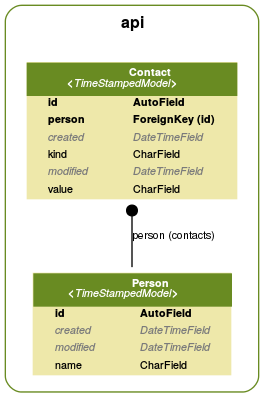
\includegraphics[width=.55\textwidth]{imagem/der.png}
    % Caption centralizada
    \captionsetup{justification=centering}
    \captionfont{\small{\textbf{\\Fonte: Autor}}}	
    \label{fig:der}
  \end{figure}

  Coforme a Figura \ref{fig:der}, os protótipos possui as seguintes tabelas: \textit{Person} e \textit{Contact},
  que fazem o registro de pessoas e contatos, respectivamente, e possui os atributos (campos) necessários
  para armazenar os registros da API no banco de dados. Na entidade de \textit{person}, temos o identificador
  "id" como chave primária, única e auto-incremento, "created" e "modified" como campos de data e o campo
  "nome" para identicar o nome da pessoa. Na tabela de \textit{contact} temos um identificador "id" único e auto-incremento,
  "created" e "modified" como campos de data, "kind" com caracter para saber o tipo do contato e "value" para 
  saber o valor do tipo do contato. A tabela \textit{contact} possui um relacionamento com a tabela \textit{person},
  com a cardinalidade de muitos para um.

  
\section{Aplicação em Django}
\label{desenvolvimento-django}

  Neste capítulo apresenta o desenvolvimento de uma aplicação Django com o pacote Django Rest Framework para que o 
  leitor tenha conhecimento geral sobre o processo de desenvolvimento com este \textit{framework}. 
  
  
\subsection{Instalação Base}

  Para iniciar o desenvolvimento com o \textit{framework} Django é necessário ter instalado no sistema operacional
  (este protótipo foi desenvolvido em Linux) as seguintes bibliotecas: python-pip; python-virtualenv; python-dev;
  libpq-dev.  O python-pip é utilizado para instalar os pacotes do repositório de pacotes do python conhecido como
  PyPI \footnote{The Python Package Index. Disponível em https://pypi.python.org/pypi}. O python-virtualenv é utilizado
  para isolar em um ambiente virtual as bibliotecas instaladas e utilizadas na aplicação para que não corrompa as bibliotecas
  do sistema operacional. O python-dev é um conjunto de ferramentas para o desenvolvimento com a linguagem python e a libpq-dev
  é a biblioteca resposável por compilar e comunicar a aplicação com o \textit{backend} do banco de dados Postgres.
  
  Após instalar essas bibliotecas no sistema operacional, deve seguir as etapas abaixo em ordem.
  
  \begin{compactitem}
    \item[1)] Criar o ambiente virtual;
    \item[2)] Instalar o \textit{framework} Django e o pacote \textit{Django Rest Framework};
    \item[3)] Criar o esqueleto ou estrutura de diretórios da aplicação.
  \end{compactitem}
  
  Para o item 1, execute o comando \textit{virtualenv django_rest}. Em seguida é necessário ativar este ambiente com o comando
  \textit{source django_rest/bin/activate}. Após a ativação do ambiente prosseguimos para segunda etapa executando o comando
  \textit{ pip install django djangorestframework}
  
  \textbf{****PRECISA FALAR DA HISTORIA DO DJANGO???? *****}
  
  O Django Rest Framework, como descrito em seu site \footnote{Disponível em http://www.django-rest-framework.org/} é uma poderosa
  e flexível caixa de ferramentas para construir APIs em aplicações Web. Dente suas facilidades pode-se destacar: navegação na API através
  de páginas html, politicas de autenticação, serialização de objetos do banco de dados, funções e classes base para prover os recursos
  de uma API e suas respectivas funcionalidades, uma extensa documentação e suporte pela comunidade.
  
  Após a visão geral do pacote, executamos a última etapa para criar a estrutura de diretórios. Para isto use o comando
  \textit{django-admin.py startproject --template https://github.com/lucassimon/django-project-template/zipball/master --extension py,md django_rest}.
  
  Com este comando ira ser criado toda a estrutura necessária para a aplicação faltando poucas alterações e configurações.
  
\subsection{Configurações}

  Entre no diretório criado e faça a instalação dos demais pacotes necessários com o comando \textit{pip install -r requirements/dev.txt}.
  Em seguida edite o arquivo \textit{settings.py} localizado dentro do diretório \textit{infra_confs/} e altere a configuração
  do nome do banco de dados na linha \textit{DATABASE_URL}.
  
  Altere o arquivo \textit{base.py} dentro do diretório \texit{django_rest/settings/} inserindo na configuração \textit{INSTALLED_APPS}
  o texto \textit{'rest_framework'}. Neste mesmo arquivo é necessário setar uma configuração do pacote Django Rest Framework
  com o objetivo de liberar a permissão de acesso para todas os recursos providos no módulo \textit{api}.
  
  92 REST_FRAMEWORK = {
  96     'DEFAULT_PERMISSION_CLASSES': [
  97     ¦   'rest_framework.permissions.AllowAny'
  98     ]
  99 }
  
  Para finalizar as configurações executamos o comando \textit{python manage.py syncdb --migrate --settings=django_rest.settings.dev}
  para sincronizar as configurações com o banco de dados criado.
  
  

\subsection{Desenvolvimento}

  Abaixo segue a metodologia e processos utilizados no desenvolvimento da API em Django.
  
  Para iniciar o desenvolvimento do protótipo é criado o módulo \textit{api}, como descrito anteriormente,
  para isto execute o comando \textit{python manage.py startapp --template https://github.com/lucassimon/django-app-template/zipball/master api}
  
  Através deste comando é criado um diretório de nome \textit{api} contendo os principais arquivos utilizados no decorrer deste protótipo.

\subsubsection{Modelos}

  Primeiro, precisa escrever o modelos através das classes \textit{Person} e \textit{Contacts}. Estas classes irão representar o diagrama
  de entidade e relacionamentos da figura \ref{fig:der}. Na classe \textit{Person} foi definido a coluna \textit{name} como um campo 
  do tipo \textit{char} e 255 caracteres.
  
  \textbf{*** AQUI ROLA DE COLAR CÒDIGO OU FIGURA???? *** }
  
  Na classe model \texit{Contact} temos o atributo prson como chave estrangeira da classe \textit{Person}, o campo \textit{kind} do
  tipo \textit{char} com no máximo 2 caracteres e o campo \textit{value}, também do tipo \textit{char} com no máximo 255 caracteres.
  
  \textbf{*** AQUI ROLA DE COLAR CÒDIGO OU FIGURA???? *** }
  \textbf{*** REPETI O QUE ESTAVA ESCRITO NO DER COMO POSSO MELHORAR??? *** }
  
  Após contruir os modelos é necessário sincronizar com o banco de dados, mas antes foi inserido o módulo \textit{api}, no 
  \textit{INSTALLED_APPS} do arquivo \textit{base.py}. Ao executar o comando \textit{python manage.py syncdb --migrate --settings=django_rest.settings.dev}
  as tabelas serão criadas no banco de dados com o sufixo \textit{api_} e o nome do model. Por exemplo \textit{api_person} e \textit{api_contact}.
  
\subsubsection{Serializidores}

  Os \textit{serializers} são parte fundamental da API pois eles irão transformar os objetos do modelo em dados JSON quando for 
  responder as requisições das URLs.
  
  Primeiro crie o arquivo \textit{serializers.py} e no ínicio do arquivo foi importado o módulo \textit{serializers} e os modelos
  criados.
  
  \textbf{*** QUE COMANDO USA NO LATEX PARA CÒDIGO *** }
  8 from rest_framework import serializers 
  11 from .models import Person, Contact
  
  Neste arquivo criou-se duas classes PersonSerializer e ContactSerializer. Ambas herdam da classe abstrada serializers.ModelSerializer.
  A classe PersonSerializer conterá a classe Meta para definir os metadados providos pela abstração do módulo ModelSerializer. Esses 
  metadados são: \textit{model} atribuíndo o modelo Person e o metadado \textit{fields} que é uma lista contendo os campos ou colunas
  do modelo a serem serializados.
  
  Para a classe ContactSerializer os metadados são: \textit{model} atribuíndo o modelo Contact e o metadado \textit{fields} com todos os
  campos deste modelo. Nesta classe foi realizado uma customização que originou um novo campo chamado \textit{kind_display}. Este campo
  tem como objetivo humanizar as opções oferecidas pelo campo \textit{kind} retornando a descrição do tipo cadastrado.

\subsubsection{Visões}

  Após ciar os modelos e os serializidores têm se de criar os \texit{endpoints} ou recursos da API. Primeiro importa os módulos
  do Django Rest Framework que são:
    
  from rest_framework.decorators import api_view
  from rest_framework.response import Response
  from rest_framework.reverse import reverse
  from rest_framework import generics
  
  É necessário importar os modelos criados e as classes de serialização dos objetos.
  
  from .models import Person, Contact 
  from .serializers import PersonSerializer, ContactSerializer
  
  As classes PersonList e ContactList herdam da classe abstrata \textit{generics.ListCreateApiView} do modulo
  importado \textit{generics} do Django Rest Framework. Essa classe abstrata possui funcionalidades implementadas para 
  listar -(metódo GET)- e criar -(metódo POST)- os objetos do banco de dados. Dentro de cada classe é necessário especificar
  nos atributos \textit{model} e \textit{serializer} correspondente a cada classe. Para a classe PersonList sera o atributo
  model será atribuito o valor do modelo Person e o atributo serializer será atribuido a classe PersonSerializer. O mesmo ocorre para 
  a classe ContactList.
  
  Para que a aplicação criada passe a responder as requisições com o metódo GET por id, PUT por id e DELETE por id é necessário criar
  as classes PersonDetail e ContactDetail. Estas classes irão herdar da classe abstrata RetriveUpdateDestroyView que ja possui 
  funcionalidades implementadas para responder essas solicitações do protocolo \ac{HTTP}.

\subsubsection{Rotas}

  Finalizando o desenvolvimento vamos ligar os modelos, serializers e views à uma rota de urls para que o usuário
  possa requisitar os dados.
  
  No arquivo urls.py crie as seguintes rotas:
  
  \begin{compactitem}
    \item[a)] url(r'^v1/pessoas/\$', PersonList.as_view(), name='person-list')
    Essa rota aponta para o endpoint PersonList e prove a listagem de pessoas com o metódo GET, como também
    provê o cadastro de uma pessoa com o metódo POST
    
    \item[b)] url(r'^v1/pessoas/(?P<pk>\d+)/\$',PersonDetail.as_view(),name='person-detail')
    Essa rota aponta para o endpoint PersonDetail e prove a listagem de uma determinada pessoa pela sua chave primária
    através do metódo GET. Com esta mesma rota é possível atualizar uma pessoa com o metódo PUT e deleta-la através do 
    metódo DELETE.
        
    \item[c)] url(r'^v1/contatos/\$',ContactList.as_view(),name='contact-list')
    Essa rota aponta para o endpoint ContactList e prove a listagem de contatos com o metódo GET, como também
    provê o cadastro de um contato com o metódo POST
    
    \item[d)] url(r'^v1/contatos/(?P<pk>\d+)/\$',ContactDetail.as_view(),name='contact-detail')
    Essa rota aponta para o endpoint ContactDetail e prove a listagem de uma determinado contato pela sua chave primária
    através do metódo GET. Com esta mesma rota é possível atualizar um contato com o metódo PUT e deleta-lo através do 
    metódo DELETE.
        
  \end{compactitem}
  

\subsection{Conclusão}

   O desenvolvimento para Django é simples e rápido. Com poucas classes e códigos ja é possível construir uma API funcional
   através do pacote Django Rest Framework. Todo o código desenvolvido fica organizado graças a obrigatoriedade de edentação
   do python.

\section{Aplicação em Express.Js}
\label{escopo-projeto}

  Falta algum texto